\section{Interaktion der Komponenten}
Auf Basis der Use Cases aus der Analyse wird in diesem Kapitel die Interaktion der einzelnen Komponenten aus Kapitel 1 betrachtet. 
Dabei liegt der Fokus vor allem auf der Interaktion zwischen dem \emph{Robot} und dem \emph{Server}, wie dessen Austausch mit dem \emph{Hospital} und der \emph{TaxiApp}. 
Die Abläufe innerhalb der Komponenten werden dann in Kapitel 8 näher spezifiziert. \\


\subsection*{Interaktion zwischen TaxiApp, Server und RobotUnit}

Elementar ist in diesem Fall der Use Case \texttt{Receive Order} (Use Case 1.1), der es Usern ermöglicht, Anfragen oder Notrufe abzusetzen, um ein Taxi oder einen Krankentransporter anzufordern. 
Das System arbeitet mit einer Warteliste für Aufträge von Taxikunden. \\
Krankentransporte werden bei der Vergabe von Aufträgen stets priorisiert und es wird ggf. ein laufender \emph{Task} eines Taxikunden unterbrochen, um einen Robot bereitzustellen. \\

Im Falle des Sequenzdiagramms aus Abbildung \ref{SequenzDiagrammInteraktionTaxi} ist dies mit der Verwendung der \emph{TaxiApp} dargestellt, die wiederum die \emph{Order} mit den Destinations an den Server weitergibt.
Danach wird vom Server überprüft, ob überhaupt Taxis verfügbar sind.
Falls keins mehr verfügbar ist, wird die Anzahl der Kunden in der Wartschlange an die App und somit an den User zurückgegeben. \\
Solange der Taxikunde noch nicht in das Taxi gestiegen ist, kann er mit \texttt{Cancel Order} (Use Case 1.2) seine Bestellung aus dem System (der Warteschlange löschen). \\

\begin{figure}[H]
	\centering
	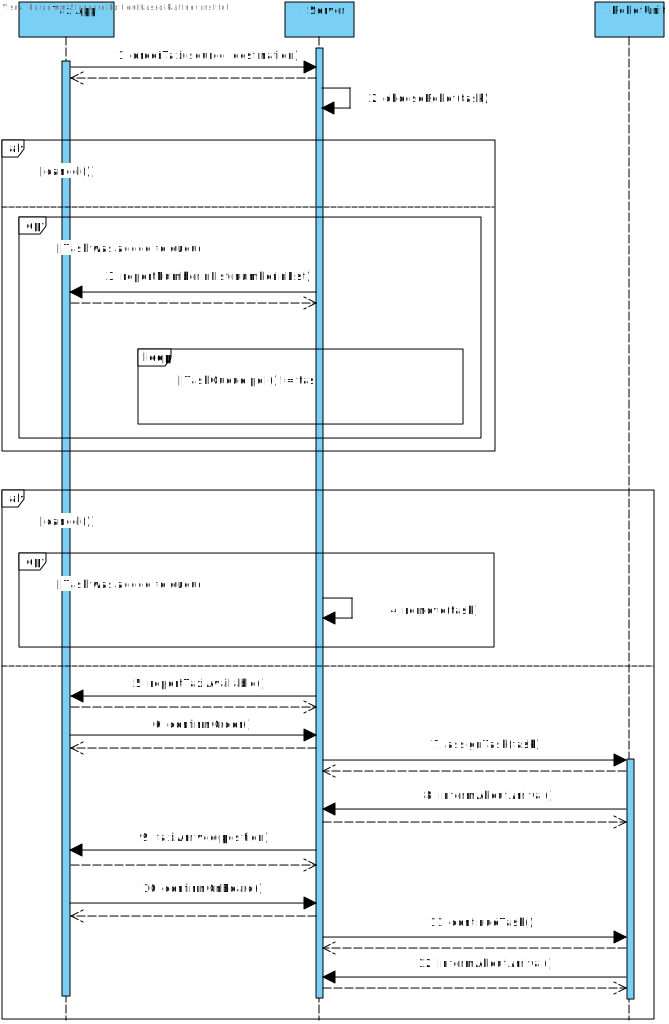
\includegraphics[width=0.9\textwidth]{img/2-Entwurf-ReceiveOrder-Taxi}
	\caption{\emph{ReceiveOrder}-Sequenzdiagramm, falls ein Kunde ein Taxi anfragt}
	\label{SequenzDiagrammInteraktionTaxi}
\end{figure}

\subsection*{Interaktion zwischen Hospital, Server und RobotUnit}

\begin{figure}[H]
	\centering
	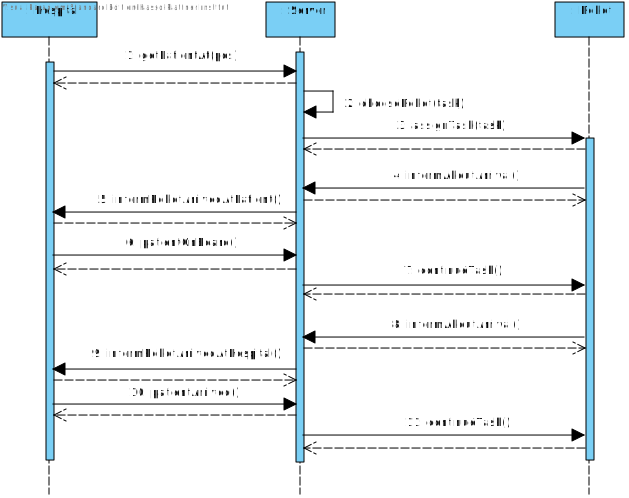
\includegraphics[width=0.9\textwidth]{img/2-Entwurf-ReceiveOrder-Hosp}
	\caption{\emph{RecieveOrder}-Sequenzdiagramm, falls das Hospital einen neuen Patienten meldet}
	\label{SequenzDiagrammInteraktionHospital}
\end{figure}


\subsection*{Kommunikation zwischen Server und RobotUnit}

\begin{figure}[H]
	\centering
	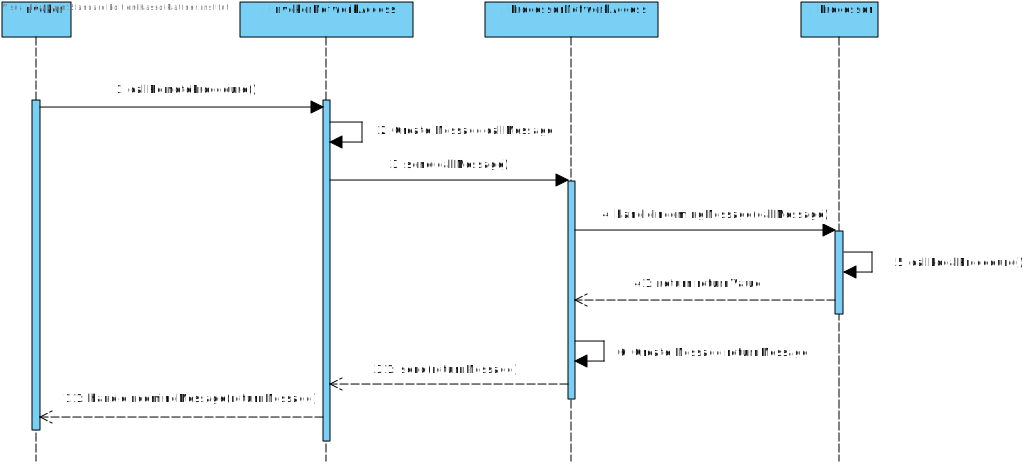
\includegraphics[width=0.9\textwidth]{img/2-Entwurf-Communication_RPC}
	\caption{Sequenzdiagramm für einen abstrakten \emph{Remote Procedure Call (RPC)}}
	\label{SequenzDiagrammRPC}
\end{figure}

